                
\onehalfspacing
%-----------------------------------------------------------------------------%
\chapter{\babSatu}
%-----------------------------------------------------------------------------%

%-----------------------------------------------------------------------------%
\section{Latar belakang}
%-----------------------------------------------------------------------------%
Bahasa merupakan representasi perilaku kompleks yang dimiliki oleh mahluk hidup dengan tingkat kognisi tinggi. Elemen bahasa seperti suara, kata-kata, dan pola sintaktis berbeda-beda untuk setiap kelompok manusia dan secara perlahan berkembang menjadi bahasa yang paling efisien \citep[p. 6]{aitchison2004change}. Hal ini disebabkan oleh berkembangnya pola linguistik seiring waktu dan penyebaran \citep{sapir1921intro}. Perkembangan ini membentuk salah satu karakteristik bahasa manusia yang paling utama, yaitu tingkat keteraturan atau organisasi isi tuturan yang sangat tinggi. Aturan-aturan ini membentuk tataran organisasi terpenting dari sebuah bahasa, yaitu sintaksis. Para linguis Jerman terdahulu menerjemahkan kata sintaksis ke dalam bahasa Jerman sebagai \textit{Satzlehre} atau 'ilmu kalimat' karena obyek dari 'sintaksis' struktural adalah studi tentang kalimat \citep{tesniere1959elements}.

Dalam kajian-kajian linguistik transformasional, para linguis memisahkan antara pengetahuan penutur terhadap sebuah bahasa untuk dapat memproduksi dan memahami bahasanya dengan bagaimana penutur menggunakan pengetahuan tersebut secara nyata untuk berbicara, memahami, membaca, dan menulis (\citealp{chomsky1965syntactic, delahuntygarvey2010soundsense}). Manusia memiliki kemampuan mental dan kognitif untuk mempelajari, memproduksi, dan mengerti ujaran yang berbeda-beda. Pengetahuan bawah sadar terhadap aturan yang membentuk sebuah bahasa ini disebut dengan 'kemampuan' (\textit{competence}). Sementara itu, aktivitas linguistik yang memanfaatkan pengetahuan tersebut secara nyata disebut dengan 'penampilan' (\textit{performance}). \cite{chomsky1965syntactic} menekankan bahwa investigasi terhadap penampilan bahasa hanya akan bermakna sejauh pemahaman terhadap kemampuan bahasa yang mendasarinya. Beberapa linguis lain seperti \cite{sagwasow2011pccg} berargumen dan mengungkapkan pentingnya penelitian mengenai penampilan bahasa yang dapat menjadi basis fakta empiris dalam perkembangan teori-teori gramatikal atau kemampuan bahasa. \cite{hawkins2014cross} juga mengeksplorasi keterkaitan antara penampilan bahasa dan konvensi tata bahasa serta mengungkapkan bahwa kecenderungan yang ditemukan dalam data penggunaan bahasa yang mencakup pilihan penutur (urutan kata, pilihan klausa, dan lain-lain) tampak serupa dengan kecenderungan yang ditemukan dalam konvensi tata bahasa. 

Tata bahasa berperan sebagai konfigurasi spesifik yang mengatur susunan unit-unit linguistik dalam sebuah kalimat. Namun, penutur yang berbeda dapat menghasilkan bentuk kalimat yang berbeda juga meskipun memiliki tata bahasa yang serupa. Hal ini diungkapkan oleh \citet[pp. 6-8]{chomsky1965syntactic} yaitu bahwa semua bahasa di dunia memiliki keserupaan dalam aspek kreatifnya. Aspek kreatif yang dimaksud adalah meskipun bahasa-bahasa tersebut memiliki aturan sintaksis yang bersifat membatasi, manusia memiliki kemampuan untuk mengekspresikan pikiran dengan jumlah variasi bentuk tuturan yang tak terhingga dan bereaksi secara tepat dalam segala bentuk situasi. Variasi bentuk tuturan hasil kemampuan pemrosesan bahasa dalam kognisi manusia ini dikaitkan dengan aspek efisiensi dalam memproduksi dan memahami sebuah kalimat.\citet[p. 231]{hawkins2014cross} menjabarkan efisiensi ini melalui dua kriteria, yaitu seberapa cepat informasi dalam sebuah kalimat diproduksi hingga diterima oleh pembaca atau pendengar dan seberapa mudah informasi tersebut diproses dalam memori kerja manusia. 

Berkaitan juga dengan efisiensi tersebut, John McWhorter menulis sebuah artikel di media daring The Atlantic \citep{mcwhorter2016efficient} dengan memaparkan beberapa bukti ujaran dari penutur bahasa Indonesia untuk menunjukkan bagaimana bahasa Indonesia merupakan salah satu bahasa paling efisien dan ekonomis. \cite{mcwhorter2016efficient} menambahkan bahwa para penutur bahasa Indonesia mengolah tata bahasanya secara alami dan berkala sehingga terdapat keteraturan bentuk bahkan dalam bahasa sehari-hari (informal). \citet[pp. 4-6]{hawkins2014cross} berasumsi bahwa aturan tata bahasa yang ada sudah memempertimbangkan keterbatasan memori kerja serta pertimbangan aspek efisiensi lain yang dikaji melalui pemanfaatan data ujaran nyata atau penampilan bahasa. Meskipun asumsi ini baru memiliki bukti kuat dalam penelitian terhadap bahasa-bahasa dengan urutan kata yang lebih tetap (\textit{fixed word order}), temuan \cite{mcwhorter2016efficient} menunjukkan indikasi bahwa gagasan hubungan tata bahasa dan efisiensi \citep[pp. 4-6]{hawkins2014cross} juga dapat terjadi pada bahasa dengan urutan kata bebas (\textit{free word order}).

Berbagai penelitian lintas bahasa telah dilakukan untuk menunjukkan bahwa banyak bahasa di dunia tidak terkekang oleh struktur urutan kata sesederhana Subyek, Predikat, dan Obyek seperti dalam Bahasa Inggris yang urutan Subyek dan Predikat-nya bisa berubah (\citealp{macwhinneybates1989cross, birnerward1998noncanonical, lambrecht2000info}). Perbedaan urutan kata dapat dimotivasi oleh berbagai aspek seperti kala waktu, kepastian, dan seberapa hidup referen sebuah nomina (\textit{animacy}) (\citealp{dryer1992greenbergian, tsunoda1995adpositions, polinskaja1989object}). \cite{hawkins1994performance} berargumen bahwa bahasa-bahasa dengan urutan kata bebas dan bahasa-bahasa dengan urutan kata tetap memiliki keterkaitan. Keterkaitan yang dimaksud adalah bahwa urutan kata yang banyak digunakan oleh penutur pada bahasa dengan urutan kata bebas memiliki kesamaan dengan urutan kata yang dikonvensionalisasikan secara aktif pada bahasa dengan urutan kata tetap. \citet[p. 110]{hawkins1994performance} menghubungkan pilihan terhadap urutan kata tertentu ke dalam asas efisiensi bahasa yang dikembangkannya dan mengatakan bahwa tipe urutan kata tertentu memudahkan pendengar memproses informasi dibandingkan tipe yang lain.

Kesimpulan bahwa bahasa Indonesia tergolong memiliki urutan kata yang bebas banyak muncul dalam penelitian mengenai urutan kata pada ranah sintaksis (\citealp{stack2005word, postman2004processing}). \citet[pp. 209-268]{sneddon2010indonesian} mengungkapkan bahwa meskipun bahasa Indonesia memiliki basis urutan kata tertentu, berbagai kondisi memungkinkannya untuk berubah. Seperti yang terjadi pada contoh perbedaan penekanan yang mengakibatkan perbedaan urutan kata antara \textit{Endang lari ke toko dengan cepat} dan \textit{Dengan cepat Endang lari ke toko}. Dalam penelitiannya, \cite{postman2004processing} menekankan bahwa bahasa Indonesia merupakan bahasa yang berorientasi pada tema sehingga tidak memiliki urutan kata yang bersifat baku atau kanonis. Urutan kata dan efisiensi kalimat dalam bahasa Indonesia ini sangat berkaitan dengan pembahasan dikotomi kemampuan dan penampilan bahasa di dunia linguistik, terutama karena bahasa Indonesia tergolong bahasa yang memiliki aturan tata bahasa yang bebas.

Selama puluhan tahun, banyak riset dilakukan untuk melihat bagaimana penutur mengatur dan memproduksi kalimat menjadi bentuk yang paling efisien (\citealp{chomsky2005three, hawkins2004efficiency, zipf1935psycho, zipf1949human}). Beberapa kajian linguistik modern yang menyoroti masalah ini memanfaatkan teori dependensi sebagai landasan teori utama. Dependensi adalah gagasan bahwa setiap unit linguistik dalam kalimat terhubung satu sama lain oleh tautan langsung karena memiliki relasi semantik \citep{tesniere1959elements}. Sebagai contoh, penutur bahasa Indonesia harus menuturkan \textit{Saya cinta kamu} dan bukan \textit{*Saya kamu cinta} seperti dalam bahasa Perancis (\textit{Je t'aime}). Hal ini memberikan gambaran hubungan struktur konstruksi kalimat dengan kerja kognisi manusia yang tidak terbatas pada satu bahasa saja \citep{gibson2000dependency}. Pada kedua kalimat tersebut, terlihat perbedaan bagaimana posisi aktor pelaku dan obyek bergantung pada proses atau verba. Contoh kasus sederhana tersebut menunjukkan bahwa kata-kata sebagai konstituen kalimat terhubung oleh tautan langsung yang disebut juga dengan dependensi (\textit{dependency}). Teori dependensi merupakan teori sintaksis modern, namun memanfaatkan konsep dasar linguistik seperti halnya konsep penanda dan petanda yang digagas oleh Saussure \citep{key2017course}. 

Menurut Saussure \citep{key2017course}, untuk dapat mengantarkan informasi tertentu, penutur harus memilih tanda pada sumbu paradigmatik dan mengatur tanda tersebut ke dalam urutan linear pada sumbu sintagmatik. Dalam teori dependensi, satu unit linguistik harus bergantung kepada unit linguistik lain untuk menempati posisi linear tertentu dan membentuk relasi sintagmatik \citep[p. 11-14]{tesniere1959elements}. Dengan kata lain, pengaturan tanda pada sumbu sintagmatik dikendalikan oleh tautan dependensi yang menghubungkan unit-unit tersebut. Perbedaan tautan-tautan dependensi dalam sebuah kalimat tidak hanya terjadi secara lintas bahasa seperti pada contoh kasus dalam bahasa Indonesia dan Perancis di atas. Dua kalimat dalam satu bahasa juga dapat memiliki pola tautan dependensi yang berbeda. Pada \pic~\ref{fig:contoh-dependensi}, kata \textit{keluar} menempati posisi pada urutan linear yang berbeda, sehingga jarak dependensi antara kata \textit{membuang} dan \textit{keluar} pada kedua kalimat juga berbeda. 
\begin{figure}
	\centering 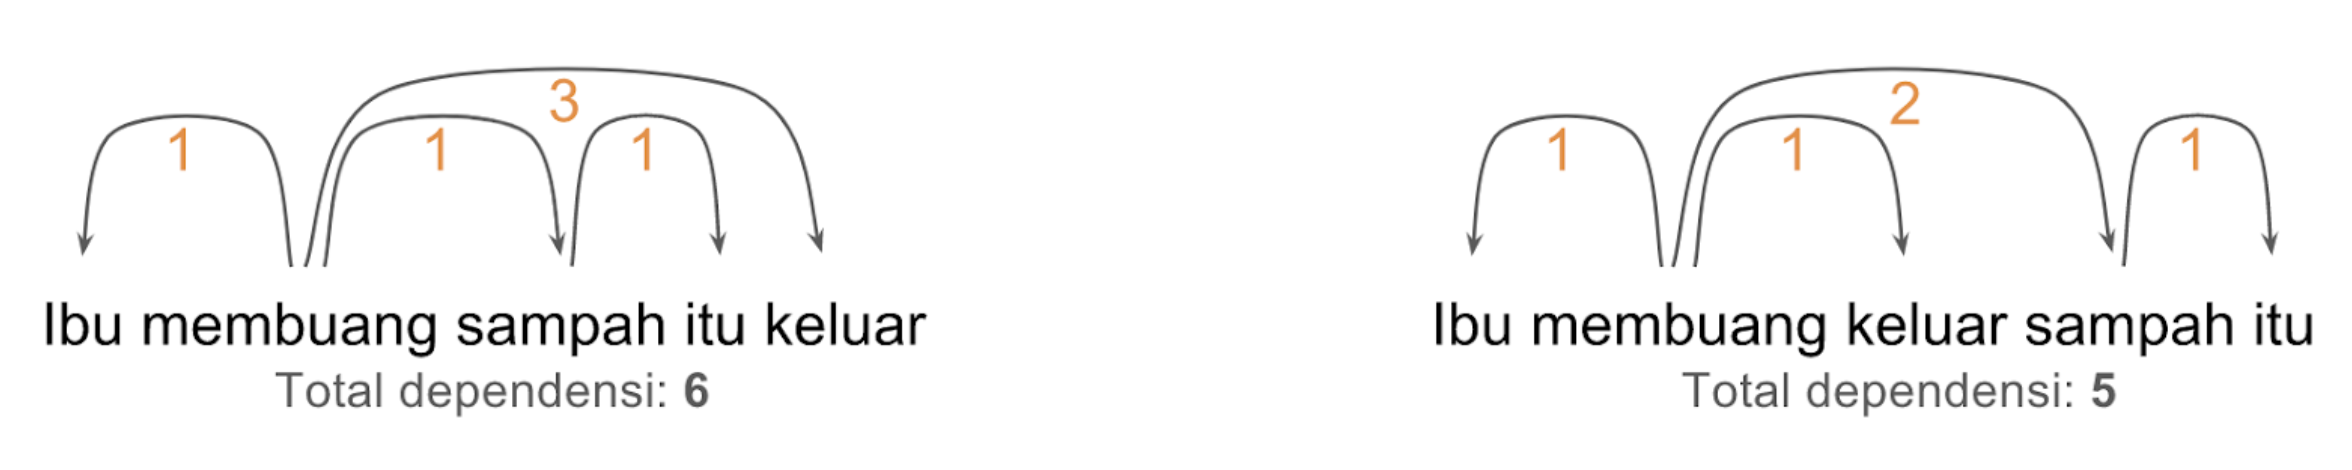
\includegraphics[width=1
	\textwidth] {pics/contoh-dependensi.png} \caption{Contoh perbedaan dependensi dalam bahasa Indonesia} 
\label{fig:contoh-dependensi} \end{figure}

Salah satu hipotesis yang membahas panjang dan jarak dependensi menyebutkan adanya kecenderungan bahwa penutur akan mendekatkan kata-kata yang memiliki relasi secara semantik dalam kalimat (\citealp{futrell2015large, liu2017dependency}). Hipotesis ini sangat berkaitan dengan prinsip efisiensi yang dikembangkan oleh \cite{hawkins2004efficiency}. Kata-kata yang mendekat mengakibatkan pengurangan panjang atau jarak dependensi sehingga berkaitan juga dengan hipotesis bahwa penutur cenderung lebih sulit dalam memproduksi dan memahami kalimat yang memiliki jarak dependensi yang jauh dan struktur yang rumit (\citealp{hawkins2004efficiency, dillon2011structured}). Sebagai contoh, pada \pic~\ref{fig:contoh-dependensi}, kata \textit{membuang} dan \textit{keluar} memiliki tautan langsung sehingga memori kerja penutur akan bekerja untuk menghubungkan keduanya. Semakin jauh jarak keduanya, semakin banyak memori kerja bekerja. Konsep tersebut mendukung penelitian \cite{jaeger2006redundancy} yang mengungkapkan bahwa penutur cenderung mengutamakan alasan efisiensi memori menyusun kata-kata dalam urutan linear pada sumbu sintagmatik, terutama pada ujaran yang lebih spontan \citep{jaeger2006redundancy}. \cite{futrell2015large} menemukan adanya fenomena pengurangan panjang dependensi antarkonstituen dalam 37 bahasa yang termasuk di dalamnya adalah bahasa Indonesia. Dalam penelitian tersebut, \cite{futrell2015large} menyebutkan bahwa temuan dalam bahasa Indonesia menunjukkan tingkat pengurangan panjang yang paling tinggi dibandingkan 36 bahasa lainnya. 

Penelitian terdahulu dengan data bahasa Indonesia yang membahas dependensi (\citealp{kamayani2011dependency, green2012indonesian, irmawati2015dependency, futrell2015large}) memanfaatkan korpus bahasa Indonesia yang mencakup data ragam tulis dari media jurnalistik daring, blog, artikel penelitian, dan media sosial. Pemilahan data dalam penelitian-penelitian tersebut hanya didasarkan pada keragaman dan kuantitas data. Berdasarkan hasil temuan \cite{wang2017effects}, \textit{genre} atau aliran teks hampir tidak berpengaruh terhadap pola distribusi jarak antarkonstituen yang memiliki relasi semantik. Hal ini berarti terlepas dari aliran teks, manusia cenderung untuk meminimalisir jarak dependensi pada kondisi tertentu \citep{wang2017effects}. Di lain sisi, \citep{wang2017effects} menemukan bahwa teks imajinatif cenderung memiliki jarak dependensi yang lebih panjang dibandingkan dengan teks informatif sehingga teks informatif lebih mudah untuk dimengerti\footnote{Penelitian \cite{wang2017effects} memanfaatkan British National Corpus yang mencakup teks informatif seperti berita dan laporan penelitian serta teks imajinatif seperti literatur fiksi dan dialog film.}. Namun, \cite{miller2011critical} mengkaji adanya perbedaan kerumitan sintaktis dalam teks informatif itu sendiri, seperti halnya media cetak formal akan lebih kompleks dibandingkan dengan artikel tabloid. Hal ini menunjukkan bahwa data penelitian linguistik terkait dependensi dapat difokuskan kepada salah satu aliran teks (informatif atau imajinatif) dan tetap mendapatkan gambaran keragaman pola yang ada di dalamnya. Keterbatasan lain yang dihadapi apabila melibatkan data bahasa sehari-hari (informal) adalah kurangnya sumber daya teknologi untuk mengolah data tersebut \citep{green2012indonesian}. 

Dalam banyaknya pembahasan mengenai efisiensi kalimat dipandang dari segi dependensi dalam linguistik secara global, terdapat kerumpangan terkait ranah tersebut dalam bahasa Indonesia. Kajian-kajian terdahulu yang menyinggung teori dependensi untuk bahasa Indonesia dilakukan oleh para peneliti terbatas untuk mengembangkan perangkat atau metode komputasional untuk penguraian kalimat berdasarkan dependensinya (\citealp{kamayani2011dependency, green2012indonesian, irmawati2015dependency}). Teori dependensi meninjau relasi semantik antara dua konstituen dalam sebuah kalimat, sehingga tidak terbatasi oleh relasi struktural. Oleh karena itu, teori dependensi merupakan dasar yang tepat untuk mengkaji ujaran nyata yang mungkin tidak memiliki struktur kalimat yang gramatikal, terutama pada bahasa-bahasa yang memiliki urutan kata bebas seperti bahasa Indonesia. Penelitian yang dapat memberikan wawasan dari aspek linguistik dengan teori dependensi akan sangat bermanfaat untuk kajian sintaksis modern terhadap bahasa Indonesia yang perkembangannya sangat alami dan cepat. Hingga saat ini, belum ada kajian dari aspek linguistik yang dapat memberikan wawasan tentang bagaimana konstruksi kalimat dapat menggambarkan efisiensi terkait panjang dan jarak dependensi dalam bahasa Indonesia. Sehubungan dengan kerumpangan tersebut, belum ada juga kajian yang memanfaatkan bukti penampilan bahasa berupa ujaran yang lebih spontan seperti data ragam lisan sebagai salah satu data utama penelitian. 

%-----------------------------------------------------------------------------%
\section{Perumusan masalah}
%-----------------------------------------------------------------------------%
Urutan kata dalam kalimat pada bahasa Indonesia tidak terkekang oleh aturan konstruksi dibandingkan dengan bahasa lain seperti Inggris dan Jerman (\citealp{stack2005word, futrell2015large, irmawati2015dependency}). \cite{kubler2009dependency} menyebutkan bahwa teori dependensi sangat sesuai untuk dimanfaatkan dalam menelaah bahasa dengan karakter urutan kata yang bebas seperti bahasa Indonesia. Tingginya tingkat pengurangan panjang dependensi kalimat yang ditemukan dalam bahasa Indonesia \citep{futrell2015large} juga menimbulkan pertanyaan mengenai keragaman pola pengurangan panjang dependensi kalimat serta jarak dependensi antarkonstituen dalam bahasa Indonesia itu sendiri.

Terkait dengan latar belakang di atas, muncul satu pokok permasalahan yang diuraikan dalam penelitian ini yaitu \textbf{bagaimana stuktur kalimat bahasa Indonesia ragam tulis dan lisan disusun secara efisien ditinjau dari segi dependensinya}. Dengan memanfaatkan korpus data jurnalistik bahasa Indonesia termutakhir ragam tulis dan lisan, pokok permasalahan ini diuraikan menjadi tiga pertanyaan yang lebih detail:

\begin{enumerate}
	\item Bagaimana pengaruh panjang kalimat terhadap penyusunan struktur kalimat yang efisien dalam bahasa Indonesia ragam tulis dan lisan dari segi dependensi? Pertanyaan ini dapat dinyatakan dalam bentuk hipotesis sebagai berikut \\
	$H_{1}A$ : Ada pengaruh panjang kalimat terhadap konstruksi kalimat dari segi dependensi. \\
	$H_{0}A$ : Tidak ada pengaruh panjang kalimat terhadap konstruksi kalimat dari segi dependensi.
	\item Bagaimana efisiensi kalimat tercermin pada panjang, jarak dan arah dependensi (direksionalitas induk) dalam bahasa Indonesia ragam tulis dan lisan? Pertanyaan ini dapat dinyatakan dalam bentuk hipotesis sebagai berikut \\
	$H_{1}B$ : Ada kecenderungan dalam bahasa Indonesia bahwa induk menempati posisi sebelum konstituen terikatnya dari segi dependensi. \\
	$H_{0}B$ : Tidak ada kecenderungan dalam bahasa Indonesia terkait posisi induk dan konstituen terikatnya.
	\item Bagaimana pengaruh penyusunan struktur kalimat yang efisien dalam bahasa Indonesia ragam tulis dan lisan dari segi dependensi terhadap valensi akar (\textit{root})?
\end{enumerate}

%-----------------------------------------------------------------------------%
\section{Tujuan penelitian}
%-----------------------------------------------------------------------------%
Penelitian ini memiliki tiga tujuan utama terkait pokok permasalahan penelitian. Pertama, penelitian ini bertujuan untuk meninjau pengaruh panjang kalimat terhadap struktur kalimat yang efisien dalam bahasa Indonesia ragam tulis dan lisan dari segi dependensi dengan memaparkan bukti empiris berdasarkan korpus data yang dikumpulkan. Kedua, penelitian ini memiliki tujuan untuk memperlihatkan bagaimana panjang, jarak dan arah dependensi (direksionalitas induk) dapat memberikan gambaran mengenai efisiensi kalimat dalam bahasa Indonesia ragam tulis dan lisan melalui analisis terhadap struktur sintaktis kalimat. Tujuan terakhir dari penelitian ini adalah untuk meninjau pengaruh struktur kalimat terhadap valensi akar (\textit{root}) kalimat tersebut dari segi dependensi.

Dalam mencapai tujuan-tujuan tersebut, beberapa aspek sintaksis terkait pembentukan struktur kalimat ini diuraikan untuk menguji hipotesis pengurangan panjang dan jarak dependensi antarkonstituen dalam sebuah kalimat seperti yang telah dibahas oleh beberapa penelitian terdahulu. Hasil penelitian ini berupa gambaran umum pengurangan panjang dan jarak dependensi pada beberapa aspek pembentukan struktur kalimat dan uraian secara mendalam mengenai tautan-tautan dependensi yang terjadi antara induk dan konstituen terikatnya. Penelitian ini menitikberatkan pada analisis penampilan bahasa (\textit{linguistic performance}) dengan memanfaatkan data penggunaan bahasa Indonesia secara nyata sebagaimana tercermin dalam korpus jurnalistik bahasa Indonesia ragam tulis dan lisan.

%-----------------------------------------------------------------------------%
\section{Manfaat penelitian}
%-----------------------------------------------------------------------------%
Jika penyusunan struktur kalimat yang digunakan penutur baik dari segi produksi maupun pemahaman didorong oleh motivasi untuk menurunkan kadar kesulitan berkomunikasi, maka ekspektasi utamanya adalah penghindaran terhadap tautan dependensi yang jauh \citep{futrell2015large}. Hipotesis pengurangan panjang dan jarak dependensi ini dapat berperan sebagai kerangka untuk menjelaskan hubungan antara bagaimana penutur memanfaatkan dan menyusun struktur sintaksis dalam sebuah bahasa dengan tujuan utama untuk menciptakan komunikasi yang efisien meskipun dengan menggunakan kalimat yang bersifat kompleks.

Secara teoretis, penelitian ini dapat menjadi dasar pengembangan ilmu sintaksis modern yang kontekstual karena menitikberatkan pada penampilan bahasa yang menjadi bukti empiris atas pemahaman kemampuan bahasa. Bukti-bukti penampilan bahasa dalam penelitian ini juga dapat ditindaklanjuti untuk merumuskan pengajaran ilmu sintaksis yang responsif terhadap penggunaan bahasa yang nyata dalam masyarakat. Selain itu, penelitian ini dapat dimanfaatkan oleh bidang perencanaan bahasa untuk memaknai penggunaan bahasa dalam masyarakat berdasarkan urutan kata dalam kalimat terkait dengan perkembangan relasi sintagmatik pada periode waktu data penelitian untuk ragam tulis dan lisan. Dalam kajian kesemestaan bahasa (\textit{language universals}), penelitian ini turut menyumbangkan gambaran mendalam terkait penampilan bahasa Indonesia dalam ranah dependensi.

Secara praktis, penelitian ini dapat memberikan kontribusi terhadap pengembangan perangkat metode linguistik komputasional dan pemrosesan bahasa alami. Kontribusi tersebut berupa wawasan tentang kajian penampilan bahasa Indonesia dalam perspektif dependensi, terutama terkait bahasa Indonesia ragam lisan yang hingga saat ini masih sangat jarang dimanfaatkan dalam pemrosesan bahasa secara digital. Temuan mengenai kaitan struktur dependensi yang memudahkan komunikasi dapat menjadi acuan utama untuk kerangka kerja dalam pemrosesan bahasa alami atau \textit{Natural Language Processing} (NLP). Seperti yang dibahas dalam penelitian \cite{klein2004corpus} serta \cite{smith2006minimum}, beberapa model komputasi termutakhir memanfaatkan asumsi pengurangan jarak dependensi untuk mereplika penggunaan bahasa oleh penutur dan hasilnya lebih mendekati ujaran nyata (\textit{real utterance}).

%-----------------------------------------------------------------------------%
\section{Batasan penelitian}
%-----------------------------------------------------------------------------%
Pada dasarnya, penelitian ini melihat bagaimana konstruksi atau struktur kalimat yang efisien dari segi dependensi. Dalam teori linguistik lain, efisiensi sebuah bahasa sering dikaitkan dengan bagaimana penutur berusaha untuk 'menghemat' tenaga dalam ujaran nyata terutama dengan memperpendek tuturan-tuturannya. Penghematan ini disebut juga dengan 'ekonomi bahasa' yang termasuk didalamnya adalah penghilangan fonem dan abreviasi \citep{verhaar1996asas}. Namun, perlu ditekankan bahwa aspek efisiensi yang dimaksud dalam penelitian ini dibatasi pada efisiensi dari segi pemrosesan terkait memori kerja pada ranah sintaksis \citep{hawkins2014cross}. Data observasi yang digunakan dalam penelitian ini merupakan kumpulan ujaran nyata yang tergabung pada korpus jurnalistik bahasa Indonesia ragam tulis dan lisan dalam rentang tahun publikasi atau rekaman dari 2008 hingga 2018. Dengan menggunakan data dari berbagai media nasional dan daerah yang menggunakan bahasa Indonesia, penelitian ini membedah struktur dan susunan kata pada tataran kalimat dengan menggunakan metode-metode yang dikembangkan berdasarkan teori dependensi yang pertama dikemukakan oleh \cite{tesniere1959elements}. 

\citet[pp. 3-5]{tesniere1959elements} menyebutkan bahwa kalimat merupakan sebuah susunan terorganisir yang memiliki konstituen berupa unit-unit kata. Organisasi konstituen dalam kalimat ini dihasilkan oleh relasi-relasi yang terbentuk antarkonstituen. Terkait dengan relasi yang muncul dalam sebuah kalimat, perlu ditekankan bahwa tidak semua relasi antarkonstituen dalam kalimat merupakan dependensi. Sebagai contoh, relasi antara kata \textit{ayah} dengan \textit{Pak Yahya} dalam kalimat \textit{Saat Budi melihat sang ayah, Pak Yahya sedang membawa adiknya pergi} bukan merupakan dependensi. Dalam kalimat tersebut, \textit{ayah} dan \textit{Pak Yahya} adalah orang yang sama sehingga memiliki relasi berupa acuan. Oleh karena itu, penelitian ini membatasi ruang lingkup relasi hanya pada relasi semantik terkait teori dependensi yang dijabarkan oleh \cite{tesniere1959elements}. Implikasi dari penelitian ini, sesuai dengan permasalahan yang diangkat, adalah pemaparan kecenderungan terkait panjang, jarak dan arah dependensi (direksionalitas induk), penelusuran pengaruh panjang kalimat terhadap strategi efisiensi kalimat dipandang dari segi dependensi, dan eksplorasi pengaruh strategi urutan kata terhadap valensi sebuah kata berdasarkan korpus yang diteliti. 

Untuk mencapai implikasi yang diharapkan, penelitian ini menggabungkan ancangan kuantitatif dan kualitatif. Ancangan kuantitatif berupa penguraian kalimat berdasarkan dependensinya (\textit{dependency parsing}), penghitungan statistika deskriptif untuk mendapatkan paparan pola struktur kalimat, dan percobaan acak dengan mengadopsi pendekatan Dasar Urutan Kata Bebas atau \textit{Free Word Order Baseline} yang digunakan oleh \cite{futrell2015large}. Penguraian kalimat berdasarkan dependensi dilakukan dengan menggunakan dasar bank pohon struktur dependensi atau \textit{dependency treebank} dalam Universal Dependencies 2.0 \citep{nivre2017universal} yang telah dikondisikan untuk bahasa Indonesia. Penghitungan statistika deskriptif untuk mendapatkan paparan pola jarak dan arah dependensi serta tes signifikansi pengaruh panjang kalimat terhadap struktur kalimat dilakukan dengan mengadopsi pendekatan yang digunakan oleh \cite{gildea2010grammars}, \cite{futrell2015large}, \cite{jiang2015effects} dan \cite{liu2017dependency}. Ancangan kuantitatif ini tidak mengukur tingkat efisiensi sebuah kalimat ataupun seberapa besar optimasi struktur sebuah kalimat dari segi pengurangan panjang dan jarak dependensi. Proses yang dibutuhkan untuk mencapai kedua tujuan ini membutuhkan pengetahuan dan metode yang berada pada ranah ilmu kognitif. Sementara itu, ancangan kuantitatif ini memiliki tujuan utama untuk untuk menguji hipotesis pengurangan panjang dan jarak dependensi pada tataran kalimat dengan memanfaatkan korpus data yang dikumpulkan dan memberikan gambaran pola-pola struktur sintaksis yang banyak muncul untuk dianalisis secara kualitatif.

Ancangan kualitatif diterapkan untuk melanjutkan hasil analisis yang didapat dari pendekatan kuantitatif. Pendekatan ini digunakan untuk menguraikan lebih dalam efisiensi kalimat terutama terkait direksionalitas induk atau  arah dependensi, perbandingan strategi struktur sintaktis pada klasifikasi berdasarkan panjang kalimat, serta struktur sintaktis kalimat yang terbentuk akibat perubahan valensi akar verbal yang diduga muncul dalam bahasa Indonesia. Seluruh ancangan kualitatif ini dilakukan pada tataran kalimat. Dalam teori dependensi, kalimat dianalogikan sebagai pertunjukan teater dengan adanya aktor (\textit{actants}), proses (\textit{verbs}), dan situasi (\textit{circumstants}) yang di setiap kalimat memiliki simpai pusat (\textit{central node}) sebagai pengendali keseluruhan kalimat \citep{tesniere1959elements}. Mengacu pada konsep ini, pendekatan kualitatif untuk melihat perubahan valensi dibatasi hanya pada simpai pusat (\textit{central node}) pada kalimat-kalimat yang mewakili pola terbanyak, yaitu kalimat yang memiliki akar berupa kata kerja atau verba. Analisis kualitatif ini menggunakan kerangka kerja tata bahasa kata (\textit{Word Grammar}) yang dikembangkan oleh (\citealp{hudson1984word,hudson2007language}). Gabungan kedua ancangan ini diharapkan dapat memberikan gambaran makro dan mikro secara sistematis dan terperinci terhadap efisiensi bahasa terkait susunan kata dalam kalimat dipandang dari segi dependensi. 



%-----------------------------------------------------------------------------%
\section{Kerangka konseptual}
%-----------------------------------------------------------------------------%
Kerangka konseptual penelitian ini melibatkan beberapa elemen dan proses mulai dari pengumpulan dan persiapan dalam membentuk korpus data ragam tulis dan lisan, pengolahan data, hingga analisis data yang melibatkan ancangan kuantitatif (percobaan acak dan agregasi data) serta ancangan kualitatif (analisis struktur sintaksis pada simpai pusat). Berikut dijabarkan keseluruhan elemen dan proses yang terlibat dalam penelitian ini:

\begin{enumerate}
	\item Data jurnalistik termutakhir dalam bahasa Indonesia yang dipisahkan menjadi kumpulan teks atau korpus (\textit{corpus}) data ragam tulis dan korpus data ragam lisan. Data jurnalistik dapat mewakili aliran penggunaan bahasa yang cukup formal untuk dapat diproses melalui metode komputasional, namun juga cukup memberikan ruang untuk penuturnya dalam berkreasi membentuk struktur kalimat tersendiri. Persiapan korpus data ragam lisan melibatkan tahapan tambahan berupa transkripsi otomatis dengan Google Speech API dan pemeriksaan secara manual untuk memastikan kualitas transkripsi. Kedua korpus juga melalui pemeriksaan secara manual untuk memastikan kalimat-kalimat tidak lengkap tidak ikut dalam proses analisis. Kedua korpus data ini merupakan masukan (\textit{input}) utama penelitian ini.
	\item Persiapan kalimat yang diekstraksi dari kedua korpus data ini merupakan tahap persiapan utama untuk dapat melalui pengolahan data dengan memanfaatkan penguraian kalimat berdasarkan dependensinya. Pemisahan ini dilakukan mengingat penelitian ini memiliki ruang lingkup pada tataran kalimat. Persiapan untuk memisahkan semua kalimat dari wacana-wacana dalam kedua korpus ini melibatkan proses otomatis dan pemeriksaan secara manual untuk memastikan kualitas data yang sesuai ekspektasi. 
	\item Ancangan kuantitatif yang melibatkan agregasi data untuk mendapatkan nilai-nilai yang dapat digunakan dalam tinjauan pengurangan panjang dan jarak dependensi serta aspek-aspek lain sesuai dengan permasalahan penelitian. Termasuk di dalam proses ini adalah percobaan acak dengan pendekatan \textit{Free Word Order Baseline} yang menjadi dasar utama pembuktian adanya pengurangan panjang dan jarak dependensi pada tataran kalimat.
	\item Ancangan kualitatif bertitik tolak dari temuan pendekatan kuantitatif yang menghasilkan indikasi-indikasi pola struktur sintaksis menggambarkan strategi untuk pengurangan panjang dan jarak dependensi. Ancangan ini melibatkan analisis terhadap struktur sintaksis kalimat dengan akar (\textit{root}) berupa verba pada simpai pusat. 
	\item Luaran dari penelitian ini berupa hasil tinjauan terhadap pengurangan panjang dan jarak dependensi serta indikasi strategi pengurangan panjang dan jarak dependensi terkait beberapa aspek struktur sintaktis. Aspek-aspek ini meliputi panjang kalimat, konstruksi kalimat yang berpengaruh terhadap panjang, jarak dan arah dependensi, serta perubahan valensi verbal pada simpai pusat.
\end{enumerate}

\newpage
Berikut adalah ilustrasi kerangka konseptual yang secara keseluruhan diterapkan dalam penelitian ini (\pic~\ref{fig:kerangka-konseptual}). 
\begin{figure}
	\centering 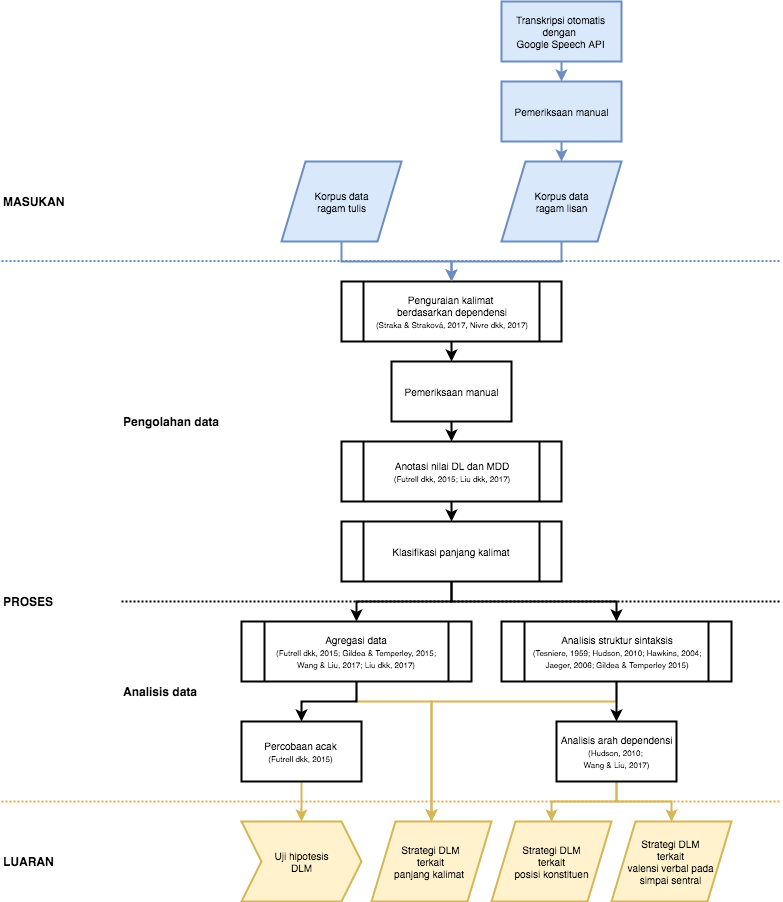
\includegraphics[width=1
	\textwidth] {pics/kerangka-konseptual.png} \caption{Diagram alur kerangka konseptual penelitian} 
\label{fig:kerangka-konseptual} \end{figure}

Berdasarkan kerangka konseptual yang telah disusun, beberapa teori dan luaran dari penelitian-penelitian terdahulu diperlukan untuk menjadi dasar kerangka teoretis penelitian tesis ini. Aspek teoretis dari kerangka konseptual tersebut dijabarkan sebagai berikut:
\begin{itemize}
	\item Spontanitas ujaran terutama dalam bahasa Indonesia menjadi dasar utama dalam menentukan jenis data yang digunakan sebagai obyek penelitian.
	\begin{itemize}
		\item Spontanitas ujaran merupakan aspek utama yang mendasari pemilihan korpus jurnalistik ragam tulis dan lisan. Dasar teoretis yang digunakan untuk mendukung perbedaan kedua ragam ini adalah variasi dan perbedaan sintaktis antara ujaran lisan dan tulisan berdasarkan pembahasan \cite{biber1991variation} dan \cite{o1974syntactic}.
		\item Teori sintaksis deskriptif yang dijabarkan oleh \cite{kridalaksana1999deskriptif, kridalaksana2002struktur} dan \textit{Indonesian Reference Grammar} \citep{sneddon2010indonesian} merupakan dasar teoretis pada aspek ketatabahasaan dalam bahasa Indonesia.
	\end{itemize}
	\item Konsep dependensi yang mendasari pendekatan penguraian kalimat berdasarkan dependensi serta penghitungan panjang dan jarak dependensi.
	\begin{itemize}
		\item Pembahasan elemen-elemen yang membentuk sebuah tautan dependensi seperti akar, induk, konstituen terikat, dan simpai menggunakan dasar teoretis dari  \cite{tesniere1959elements} yang kemudian dikembangkan oleh \cite{heringer1993dependency} dan \cite{hudson2010introduction}.
		\item Indikator panjang dan jarak dependensi yang dikembangkan oleh \cite{liu2017dependency} dan \cite{gildea2010grammars} menjadi dasar pembahasan untuk kuantifikasi atau penghitungan tautan dependensi dan anotasi panjang dan jarak dependensi pada setiap kalimat.
		\item Beberapa luaran penelitian yang dilakukan oleh \cite{gibson1998linguistic}, \cite{hiranuma1999syntactic}, \cite{liu2009chinese}, dan \cite{wang2017effects} mengenai pengaruh panjang kalimat dan jenis teks terhadap dependensi digunakan sebagai acuan klasifikasi kalimat terkait faktor-faktor yang mempengaruhi tautan dependensi.
	\end{itemize}
	\item Dasar proses analisis untuk melihat efisiensi kalimat dari segi dependensi melalui percobaan acak dan analisis kualitatif struktur sintaktis yang telah diuraikan berdasarkan dependensinya.
	\begin{itemize}
		\item Pengurangan panjang dependensi (\citealp{temperley2007minimization, temperley2008dependency, gildea2010grammars}), pengurangan jarak dependensi (\citealp{liu2008dependency, liu2017dependency}) dan pembahasan efisiensi kalimat terkait memori kerja \citep{hawkins2004efficiency} digunakan sebagai hipotesis yang mendasari analisis efisiensi kalimat dari segi dependensi melalui percobaan acak.
		\item Beberapa dasar teoretis digunakan sebagai dasar analisis kualitatif terhadap tautan dependensi mengenai tingkat kedalaman struktur sintaktis \citep{yngve1960model}, posisi induk terhadap konstituen terikat atau direksionalitas induk (\citealp{dryer1992greenbergian, temperley2008dependency}), dan valensi pada simpai pusat akar verbal (\citealp{hudson2007language, welke2002deutsche})
	\end{itemize}
\end{itemize}
	
%-----------------------------------------------------------------------------%

